
\section{String similarity joins with taxonomy}


We extend our definition to composite relation. For example: ''U.S and China'' is a composite hyponym of ``California and Beijing''. Another example: ``Hong Kong and California'' and ``U.S.''. This is a partial hypernym relation, since only California is a hypernym of U.S.

The sort-merge algorithm cannot work here.

Labeling scheme and the join:

If there are more than one string, then we can perform the verification after the filtering.


 Therefore, we propose a labeling scheme to process. Convert it to the ancestor-descendant joins



\subsection{Similarity measures}



We define the taxonomy similarity between two strings:

\begin{definition}[Taxonomy intersection]
Given two token sets $S_1$ and $S_2$, and a taxonomy $\mathcal{T}$, we say an element (token) $e \in S_1 \bigcap_T S_2$ if one the following cases is satisfied:

(1) $ e \in S_1$ (resp. $S_2$) and $\exists t \in S_2$ (resp. $S_1$), s.t. $(e,t) \in \mathcal{T} $, or

(2) $ e \in S_1$, and $e$ is a token of $e'$, and every token $e''$ in $e$ is in the set $S_1$, s.t. $\exists (e',t) \in \mathcal{T}$.\end{definition}

\begin{definition}[Taxonomy similarity]   Given two sets of tokens $S_1$ and $S_2$,we define the taxonomy similarity (TS) between $S_1$ and $S_2$ as follows:

\begin{equation}
TS(S_1,S_2)=  \frac{(S_1 \bigcap_T S_2) \bigcup (S_1 \bigcap S_2) }{S_1 \bigcup S_2}
\end{equation} \end{definition}

\subsection{String similarity join algorithms}


%\begin{figure}[t]
%\centering
%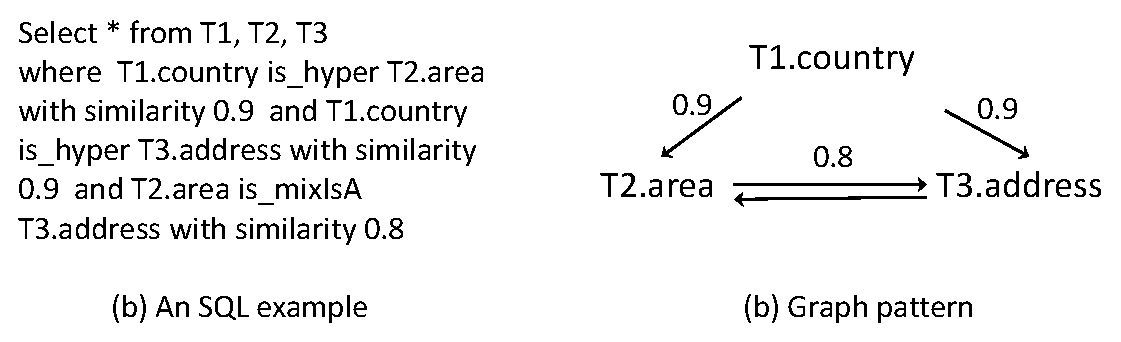
\includegraphics[scale=0.4]{figures/tgsql2}
% \caption{Taxonomy graph example }
%\label{fig:similaritygeaph}
%\end{figure}



\textbf{Baseline algorithm}. We can use the similar algorithm as that in string exact join with taxonomy. And then use these candidate for filtering. But this baseline algorithm has one limitation that there are too many candidates. Then we show how to perform the second filtering to reduce the number of candidate pairs.

\textbf{Signature-based index}. Given a string s with length $|s|$, then the size of signature is $\lceil (1-\theta)|s| \rceil$. But if the signatures involve the taxonomy, then we cannot make this argument.

But if in some real cases, we select the word from taxonomy as signatures. Therefore we need to compute a relax maximum similarity. In this case, we still do not need to retrieve the whole string to compute real similarity.

Given as string $s$, assume that its applied taxonomy node is $n$.

In this paper, we propose a new index which combine a signature filters and a length together with a bit-matrix, which extends bloom filter to two dimensions.

In the literature, the current "modus operandi" is called \textit{prefix filter}, which is based on the intuition that if two canonicalized records are similar, some fragments of them should overlap with each other, as otherwise the two records
won't have enough overlap. This intuition can be formally captured by the prefix-filtering
principle \cite{conf/icde/ChaudhuriGK06} rephrased below.

\begin{lem} (\textsc{Prefix filter principle}) \cite{conf/icde/ChaudhuriGK06} Given an
ordering $O$ of the token universe $U$ and two strings $s$ and $t$, each with tokens sorted in the
order of $O$.   If Jaccard($s, t$) $\geq \theta$, then the first $\lceil(1-\theta)|s|\rceil$ smallest
tokens of $s$ and the first $\lceil(1-\theta)|t|\rceil$ smallest
tokens of $t$  must share at least one token.
\end{lem}

%\subsubsection{Bloom matrix}
%
%We develop a new bloom matrix to extend the bloom filtering to quickly decide if there are any possibility that two sets of collections can produce at least one matching pair.
%
%There are three conditions
%
%(1) There are no overlapping for non-taxonomy bloom matrixes.
%
%(2) No taxonomy relationships and no signature bloom filter with taxonomy tokens.
%
%(3) Length filtering for those taxonomy strings.
%
%If (1) and (3) OR (1) and (2) are satisfied, then there are no any solution. We can quickly skip the join for those two collections. Otherwise we need to go into the collection and use the following algorithm to find the join solutions.


\subsubsection{Composite signature filtering}


Given a string s=\{A,B,C,D,E\}. If we use the prefix filtering, then the signature is A and B. Assume that $\theta$=0.75, (1-0.75)*5=1.25 and $\lceil 1.25 \rceil$=2. But in our bi-tuple scheme, we select two tokens as the signatures, including \{A,B\},\{A,C\},\{B,C\}.

Similarly, we can develop a 3-tuple signature. we select three tokens as the signatures, including $\binom{4}{3}$=4, i.e. \{A,B,C\}, \{A,C,D\}, \{B,C,D\}, \{A,B,D\}.

Furthermore, we can extend to 4-tuple signature, that is $\binom{5}{4}$=4, i.e. \{A,B,C,D\}, \{A,C,D,E\}, \{A,B,D,E\}, \{A,C,D,E\}, \{B,C,D,E\}.

One question is how to select the number $n$ for n-tuple scheme. What is the optimal value of $n$?

Given a string s with length $|s|$, assume that we use n-tuple signature, and the similarity threshold is $\theta$.

Then the number of signature is  $\binom{(1-\theta)|s|+n-1}{n}$ = $O(((1-\theta)|s|+n-1)^{n})$

Let $t= (1-\theta)|s|$, that is, $O((t+n-1)^{n})$. If n is too large, then there are many signatures, it may not be an optimal solution. Therefore, the key point is how to decide a good $n$?

\smallskip

\noindent \textbf{Composite signatures.} That means, the signatures may contain both TG IDs and tokens. We describe our methods as follows:

 Given a string s=\{A,B,C,D,E\}, assume that we use 3-tuple signature, $\binom{4}{3}$=4, i.e. \{A,B,C\}, \{A,C,D\}, \{B,C,D\}, \{A,B,D\}.

For each tokens, there are two cases, that is, it contains a taxonomy word, say $t \in w$. Then we use $w$ to replace $t$. Note that $t$ may belong to multiple taxonomy words. Therefore, ($w_1, w_2, \cdots, w_3$)

Continue the above example, assume that $AB$ = 1.1, $BE$= 2.3. Note that $E \in s $, but $E$ does not belong to the signatures. Then the new four signatures: \{A,B,C\}, \{1.1,C\}, \{2.3,A,C\}, \{A,C,D\}, \{1.1,C,D\},\{B,C,D\},  \{2.3,C,D\}, \{A,B,D\}, \{1.1,D\}, \{2.3,A,D\}.

\subsubsection{Comparison with other schemes}

 We compare our composite prefix filter with state-of-the-art filters. The objective of the filters is to prune dissimilar strings as many as possible. They require to select a set of q-grams from each of two strings as signatures, denoted as Sig(r) and Sig(s), and compare the two q-gram sets to check whether they share common signatures. Pruning power and filtering cost are two important issues in designing filters.

We first consider the pruning power. One one hand, the smaller the production size of the two signature sets $|Sig(r)| \times$
$|Sig(s)|$, the smaller probability they share common q-grams, and thus the higher pruning power. On the other hand, the number of matching q-grams cannot exceed the smaller signature size of the two strings, min($|Sig(r)|, |Sig(s)|$). Thus
we can use the production size of two signature sets and
the smaller signature set size to evaluate the pruning power. We then evaluate the filtering cost. As the q-gram sets
are sorted, we can use a merge-join algorithm to find the
matching q-grams if there is no index, the filtering cost depends on the sum of signature set sizes of the two strings,
$|Sig(r)|$ + $|Sig(s)|$. Table 3 compares the pruning power and filtering cost of state-of-the-art q-gram-based filters used in AllPair, ED-Join, Qchunk-IndexChunk and Qchunk-IndexGram.

\smallskip

\noindent \textbf{Length filters}


\subsubsection{Composite signature: Performance}

In this section, we cover various aspects of Composite-signature scheme's performance.
We begin by proving that it has good asymptotic performance: For a particular setting of n1 and n2, we can prove
that it provides good filtering effectiveness (i.e., generates only a few false positive candidate pairs) with few signatures per input set.

\begin{theorem} If the Jaccard similarity of two strings are greater than $\theta$, then $Sig(u) \bigcap Sig(v) = \varnothing$ with probability 1-o(1). For this setting of parameters, the number of signature per string is O().
\end{theorem}

\subsection{Count-Min estimation}

In order to quickly decide if the number of pairs after composite filters, we develop a count-min estimation to quickly determine which $n$ is good for filtering. See the following two examples for joins.

See the example in Figure \ref{fig:signature_example1}. In this example, $\theta$ = 0.8. If we use the 1-element signature, then we cannot prune away any string pair. In signature 2, we use 2-element signature, then there is no candidate. Therefore, the filtering power is better.

Further, when we consider the taxonomy ABCD ISA AGK, shown in Figure \ref{fig:signature_example1}. Then there is one answer pair (s1,t1). The new signature include the taxonomy ID 1.1 and 1  as shown.

\begin{figure}[h]
\centering
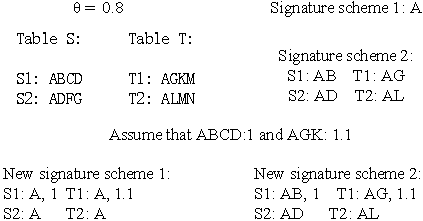
\includegraphics[scale=0.8]{figures/signature_example1}
 \caption{Illustration to the difference of signature schemes}
\label{fig:signature_example1}
\end{figure}

A Count-Min (CM) sketch with parameters ( $\varepsilon, \delta$) is represented by a two-dimensional
array counts with width $w$ and depth $d$. Given parameters ($\varepsilon, \delta$), set
$w$ = $\lceil \frac{e}{\varepsilon} \rceil$ and $d$ = $\lceil ln \frac{1}{\delta} \rceil $. Each entry of the array is initially zero.


When a data item ($w,i$) arrives, meaning that the signature $w$ has the length $i$, then $i$ is added to one cell in each row; the counter is determined by $h_j$. Formally, set $\forall 1 \leq j \leq d$, then count[j,$h_j(i)$]


The space used by Count-Min sketches is the array of $wd$ counts, which takes $wd$ words, and $d$ hash
functions, each of which can be stored using 2 words when using the pairwise functions described in [27].

Estimation procedure. Our estimation for $S \bigodot T $ = $min_j S_j \bigodot T_j $


\begin{theorem}
With a probability 1- $\delta$, The upper bound and lower bound of Composite signature estimation is
 $S \bigodot T $ and  $S \bigodot T $ + $\varepsilon |S| |T|$, respectively.
\end{theorem}

\begin{theorem}
Our composite signature estimation estimates the lower and upper bounds of algorithms by keeping space $O(\frac{1}{\varepsilon} \log \frac{1}{\delta})$ and
\end{theorem}

\subsubsection{Estimation with length filters}

When we use the CountMin sketch to estimate the effectiveness of length filter. It is to

%We  demonstrate that the returned lower and upper bounds are correct, and then we analyze its space and time complexities.
%
%Given a bucket with the sum $S$ and the number of lengths is $n$, the maximal frequency is $Max$, and the minimal frequency is $Min$, Suppose each element can join with other adjacent $\mu$ elements.
%
%Let $t = \frac{S}{M}$. Without the loss of generality, we assume that $t_1 \geq t_2$. Therefore, the upper bound of the join size is:
%
%$t_2 \times \mu M_1 M_2$ + $(t_1-t_2) \times \mu M_1$ = $\mu M_1 S_2$.
%
%In other words:
%
%$max(S_1 \cdot M_2, S_2 \cdot M_1)$
%
%The lower bound of the join size is
%
%$\mu \cdot (S_1+ S_2)$
%
%When we separate the data to two parts, we can try to make them the same for the sum.
%
%\begin{theorem} With at most $O(\log N)$ storage, we can compute the approximation with length filter. Each new data item needs $O(\log N)$ time to be processed.
%\end{theorem}




